In this chapter I present experiments performed by myself and others, examining the \alg{BOSS} and \alg{BFS3} algorithms, and comparing them to other algorithms in the same spirit.

\section{BOSS experiments}

The algorithm \alg{BOSS}, or \alg{Best Of Sampled Set}, is discussed in detail in Chapter~\ref{sec:boss}.

\subsection{Chain}


Consider the well-studied 5-state chain
% dearden98
problem (\env{Chain})~\cite{strens00,poupart06}.  The agent has two
actions: Action~1 advances the agent along the chain, and Action~2
resets the agent to the first node.  Action~1, when taken from the
last node, leaves the agent where it is and gives a reward of 10---all
other rewards are 0.  Action~2 always has a reward of 2.  With
probability $0.2$ the outcomes are switched, however.  Optimal
behavior is to always choose Action~1 to reach the high reward at the end
of the chain.

% 2-cluster 5 state chain
%  k
%  1 2977.86  21.1665
%  2 3019.04  23.0291
%  5 3036.252 22.2821
% 10 3080.652 20.8937
% 15 3030.116 19.2869
% 20 3077.132 17.3628
% 1 and 10, p = 0.000570

The slip probability $0.2$ is the same for all state--action pairs.
Poupart~et~al.~(2006) consider the impact of encoding this constraint
as a strong prior on the transition dynamics.  That is, whereas in the
\prior{Full} prior, the agent assumes each state--action pair corresponds
to independent multinomial distributions over next states, under the
\prior{Tied} prior, the agent knows the underlying transition dynamics
except for the value of a single slip probability that is shared
between all state--action pairs.  They also introduce a \prior{Semi} prior
% that is similar to \prior{Tied} except that 
in which the two actions have independent slip probabilities.
Posteriors for \prior{Full} can be maintained using a Dirichlet (the conjugate
for the multinomial) and \prior{Tied}/\prior{Semi} can be represented with a simple
Beta distribution.

In keeping with published results on this problem, Table~\ref{t:chain}
reports cumulative rewards in the first 1000 steps, averaged over 500
runs.  Standard error is on the order of 20 to 50.  The optimal policy
for this problem scores 3677.  The \alg{exploit} algorithm is one that
always acts optimally with respect to the average model weighted by
the posterior.  \alg{RAM-RMAX}~\cite{leffler07} is a version of \alg{RMAX} that
can exploit the tied parameters of tasks like this one.  Results for
\alg{BEETLE} and \alg{exploit} are due to Poupart~et~al.~(2006).  All runs used a
discount factor of $\gamma=0.95$ and \alg{BOSS} used $B=10$ and $K=5$.

\begin{table}
\caption{Cumulative reward in \env{Chain}~\cite{asmuth09}}
\label{t:chain}
\center{\small
\begin{tabular}{lcccr}
        & \prior{Tied} & \prior{Semi} & \prior{Full} \\
\alg{BEETLE} &  3650 & 3648 & 1754 \\
\alg{exploit} & 3642 & 3257 & 3078 \\
\alg{BOSS} &        3657 & 3651 & 3003 \\%  & 3611\\
\alg{RAM-RMAX} &    3404 & 3383 & 2810
\end{tabular}
}
\end{table}

All algorithms perform very well in the \prior{Tied} scenario (although
\alg{RAM-RMAX} is a bit slower as it needs to estimate the slip probability
very accurately to avoid finding a suboptimal policy).
Poupart~et~al.~(2006) point out that \alg{BEETLE} (a belief-lookahead
approach) is more effective than \alg{exploit} (an undirected approach) in
the \prior{Semi} scenario, which requires more careful exploration to perform
well.  In \prior{Full}, however, \alg{BEETLE} falls behind because the larger
parameter space makes it difficult for it to complete its
belief-lookahead analysis.

\alg{BOSS}, on the other hand, explores as effectively as \alg{BEETLE} in \prior{Semi},
but is also effective in \prior{Full}.  A similarly positive result (3158) in \prior{Full} is
obtained by \alg{Bayesian DP}~\cite{strens00}.

\subsubsection{BAYESIAN MODELING OF STATE CLUSTERS}
\label{s:cluster}

The idea of state clusters is implicit in the \prior{Tied} prior.
%  from the previous section.  
We say that two states are in the same cluster if
their probability distributions over relative outcomes are the same
given any action.  In \env{Chain}, for example, the outcomes are advancing along the
chain or resetting to the beginning.  Both actions produce the
same distribution on these two outcomes independent of state, Action~1
is 0.8/0.2 and Action~2 is 0.2/0.8, so \env{Chain} can be viewed as a
one-cluster environment.

We introduce a variant of the chain example, the two-cluster \env{Chain2},
which includes an additional state cluster.  Cluster~1---states 1, 3,
and 5---behaves identically to the cluster in Chain.
%  (0.8/0.2, 0.2/0.8).  
Cluster~2---states 2 and 4---has roughly the reverse
distributions (Action~1 0.3/0.7, Action~2 0.7/0.3).

\alg{RAM-RMAX} can take advantage of
cluster structure, but only if it is known in advance.  In this
section, we show how \alg{BOSS} with an appropriate prior can learn an
unknown cluster structure and exploit it to speed up learning. The prior used is the \prior{cluster} prior, defined in Chapter~\ref{sec:models}.


We ran \alg{BOSS} in a factorial design where we varied the environment
(\env{Chain} vs.\ \env{Chain2}) and the prior (\prior{Tied}, \prior{Full}, vs.\ \prior{Cluster}).  For our
experiments, \alg{BOSS} used a discount factor of $\gamma = 0.95$,
knownness parameter $B=10$, and a sample size of $K=5$.  The
\prior{Cluster} CRP used $\alpha=0.5$ and whenever a
sample was required, the Gibbs sampler ran for a burn period of 500
sweeps with 50 sweeps between each sample.

\begin{figure}[t]
\begin{center}
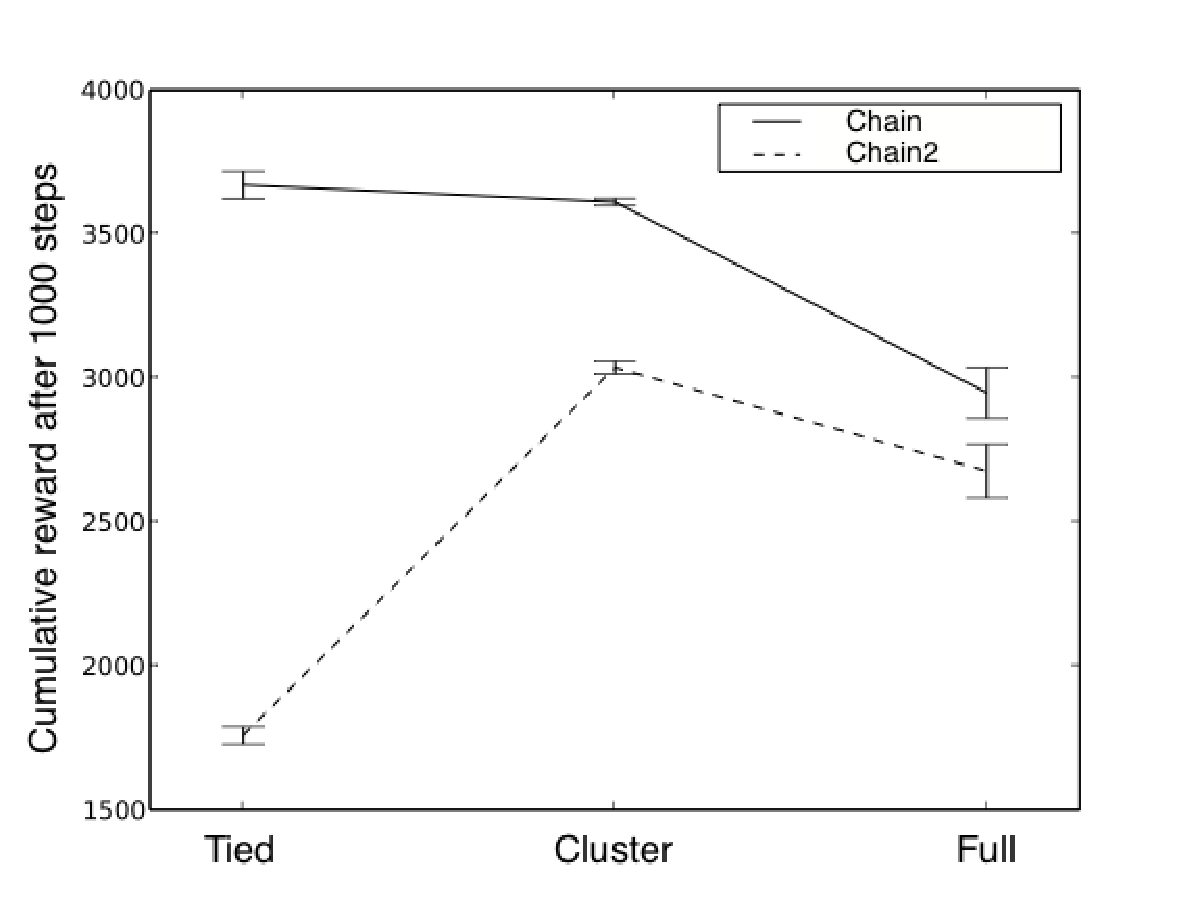
\includegraphics[width=1.0\linewidth]{2x3}
\caption{Varying priors and environments in \alg{BOSS}.}
\label{f:twobythree}
\end{center}
\end{figure}

Figure~\ref{f:twobythree} displays the results of running \alg{BOSS} with
different priors in \env{Chain} and \env{Chain2}.  The top line on the graph
corresponds to the results for \env{Chain}.  Moving from left to right, \alg{BOSS}
is run with weaker priors---\prior{Tied}, \prior{Cluster}, and \prior{Full}.  Not
surprisingly, performance decreases with weaker priors.
Interestingly, however, \prior{Cluster} is not significantly worse than
\prior{Tied}---it is able to identify the single cluster and learn it quickly.

The second line on the plot is the results for \env{Chain2}, which has two
clusters.  Here, \prior{Tied}'s assumption of the existence of a single
cluster is violated and performance suffers as a result.  \prior{Cluster}
outperforms \prior{Full} by a smaller margin, here.  Learning two independent
clusters is still better than learning all states separately, but the
gap is narrowing.  On a larger example with more sharing, we'd expect
the difference to be more dramatic.  Nonetheless, the differences here
are statistically significant ($2\times 3$ ANOVA $p<0.001$).


\subsubsection{VARYING $K$}

The experiments reported in the previous section used model samples of
size $K=5$.  Our next experiment was intended to show the effect of varying the
sample size.  Note that \alg{Bayesian DP} is very similar to \alg{BOSS} with $K=1$,
so it is important to quantify the impact of this parameter to
understand the relationship between these algorithms.

Figure~\ref{f:varyk} shows the result of running \alg{BOSS} on \env{Chain2} using
the same parameters as in the previous section.  Note that performance
generally improves with $K$.  The difference between $K=1$ and $K=10$ is
statistically significant (t-test $p<0.001$).

\begin{figure}[t]
\begin{center}
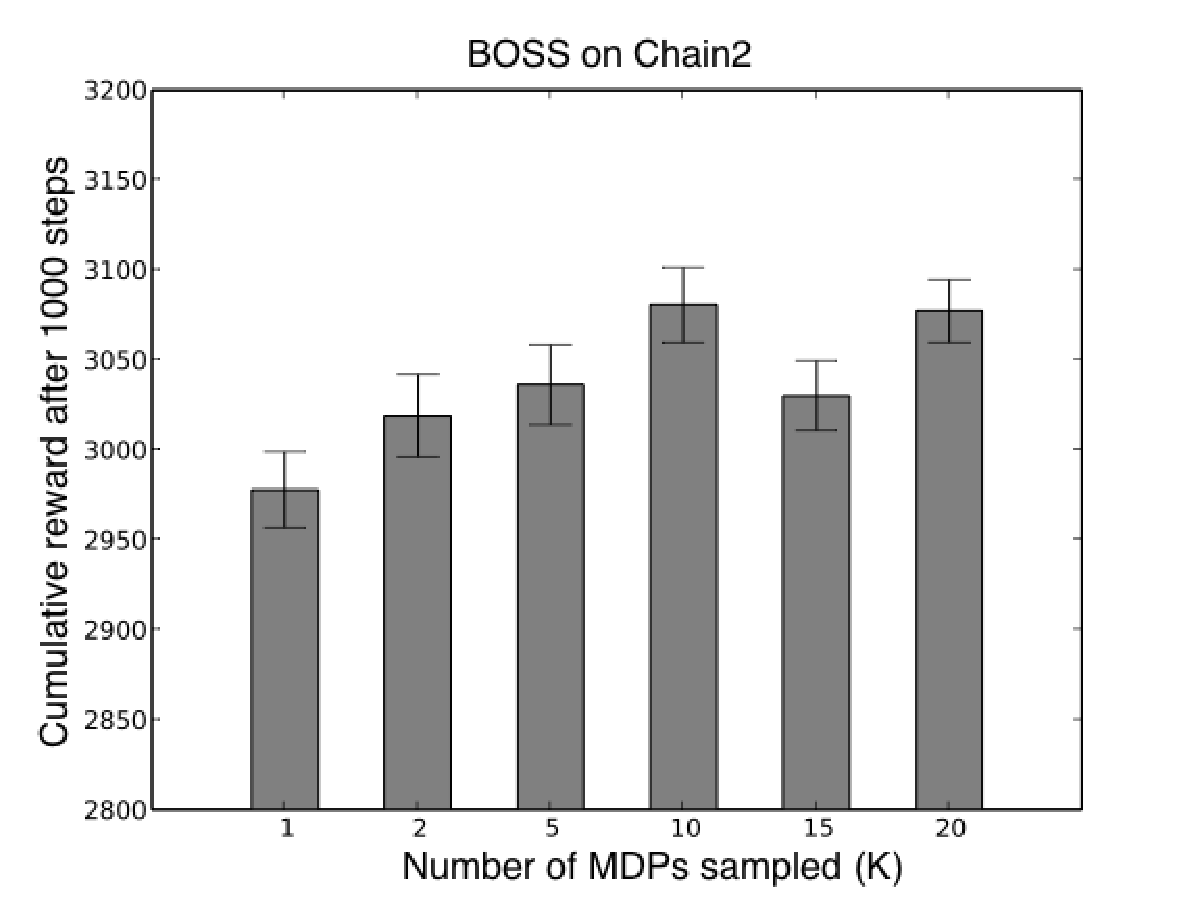
\includegraphics[width=1.0\linewidth]{varyk}
\caption{Varying $K$ in \alg{BOSS}.}
\label{f:varyk}
\end{center}
\end{figure}


\subsection{\env{Marble Maze}}


To demonstrate the exploration behavior of our algorithm, we developed a
6x6 grid-world domain with standard dynamics~\cite{russell94}.  In this environment, the four actions,
\emph{N}, \emph{S}, \emph{E} and \emph{W}, carry the
agent through the maze on its way to the goal.  Each action has its
intended effect with probability .8, and the rest of the time the
agent travels in one of the two perpendicular directions with
equal likelihood.  If there is a wall in the direction the agent tried
to go, it will remain where it is.  Each step has a cost of $0.001$, and
terminal rewards of $-1$ and $+1$ are received for falling into a pit or
reaching the goal, respectively.  The map of the domain, along with
its optimal policy, is illustrated in Figure~\ref{f:marble}.

\begin{figure}[t]
\begin{center}
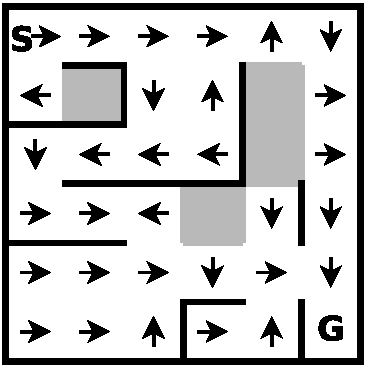
\includegraphics[width=0.6\linewidth]{6x6_maze}
\caption{Diagram of \env{6x6 Marble Maze}.}
\label{f:marble}
\end{center}
\end{figure}

The dynamics of this environment are such that each local pattern of
walls (at most $16$) can be modeled as a separate cluster.  In fact,
fewer than 16 clusters appear in the grid and fewer still are likely
to be encountered along an optimal trajectory.  Nonetheless, we
expected \alg{BOSS} to find and use a larger set of clusters than in the
previous experiments.

For this domain, \alg{BOSS} used a discount factor of $\gamma=0.95$ and a
CRP hyperparameter of $\alpha=10$.  Whenever an MDP set was needed,
the Gibbs sampler ran for a burn period of 100 sweeps with 50 sweeps
between each sample.  We also ran \alg{RMAX} in this domain.

% Figure~\ref{f:marblegraph} presents the results. 
The cumulative
reward achieved by the \alg{BOSS} variants that learned the cluster
structure, in Figure~\ref{f:marblegraph}, dominated those of \alg{
RMAX}, which did not know the cluster
structure.  The primary difference visible in the graph is the time
needed to obtain the optimal policy.  Remarkably, \alg{BOSS} $B=10$ $K=10$
latches onto near optimal behavior nearly instantaneously whereas the
\alg{RMAX} variants required 50 to 250 trials before behaving as well.
This finding can be partially explained by the choice of the clustering prior
and the outcomes it drew from, which effectively put a lower bound on
the number of steps to the goal from any state.  This information made it easy for
the agent to ignore longer paths when it had already found something that
worked.

\begin{figure}[t]
\begin{center}
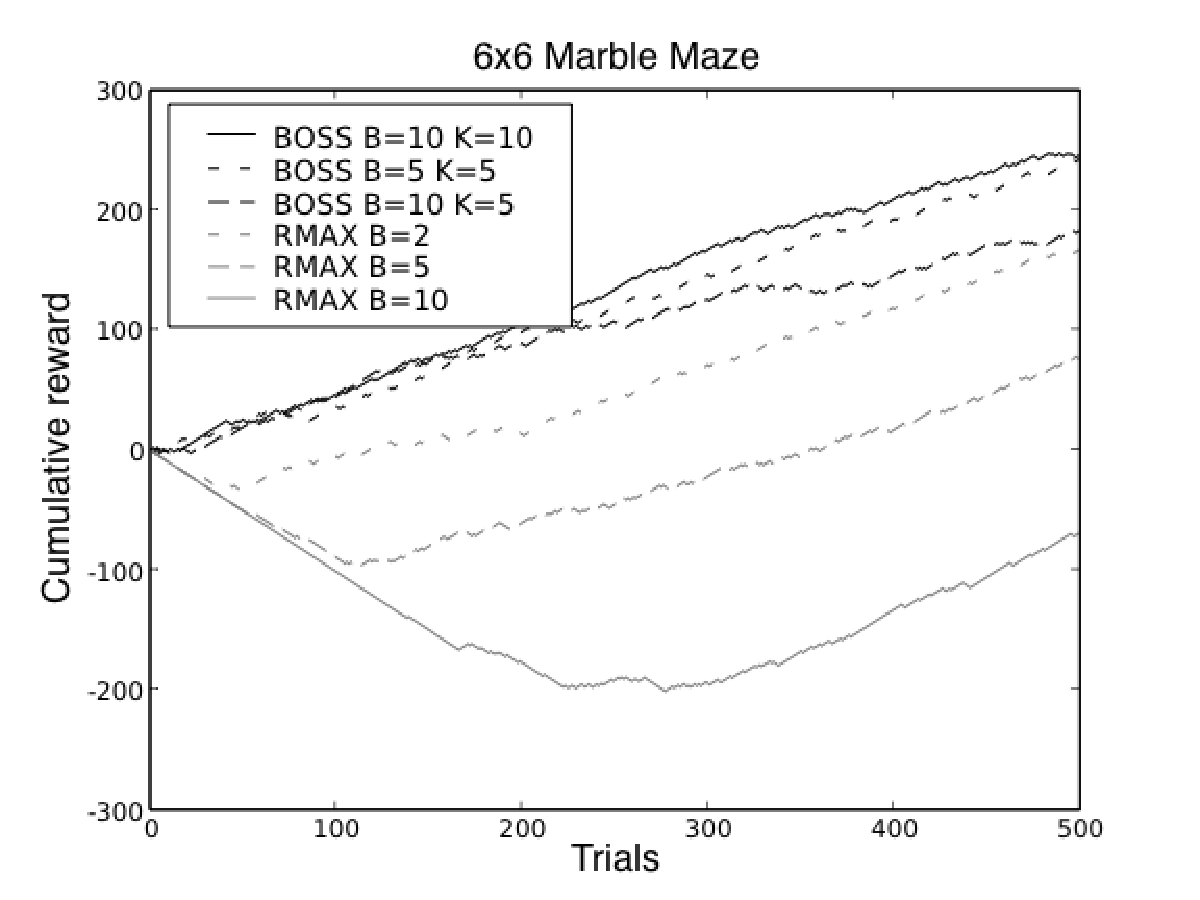
\includegraphics[width=1.0\linewidth]{marblemaze}
\caption{Comparison of algorithms on \env{6x6 Marble Maze}.}
\label{f:marblegraph}
\end{center}
\end{figure}

Looking at the clustering performed by the algorithm, a number of
interesting features emerge.  Although it does not find a one-to-one
mapping from states to patterns of walls, it gets very close.  In
particular, among the states that are visited often in the optimal
policy and for the actions chosen in these states, the algorithm
groups them perfectly.  The first, third, fourth, and fifth states in
the top row of the grid are all assigned to the same cluster.  These
are the states in which there is a wall above and none below or right,
impacting the success probability of \emph{N} and \emph{E}, the two actions
chosen in these states.  The first, second, third, and fifth states in
the rightmost column are similarly grouped together.  These are the
states with a wall to the right, but none below or left, impacting the
success probability of \emph{S} and \emph{E}, the two actions chosen in these
states.  Other, less commonly visited states, are clustered somewhat
more haphazardly,
%  It is possible that they would become more accurate
% in a longer run, but 
as it was not necessary to visit them often to
obtain high reward in this grid.  The sampled models used around
10~clusters to capture the dynamics.

\subsection{\env{Puddle World}~\cite{boyan94b}}
\label{puddle}

\env{Puddle World} is an RL benchmark in which an agent attempts to navigate two-dimensional space using four actions equivalent to \emph{north}, \emph{east}, \emph{south} and \emph{west}. The outcome dynamics are consistent across the entire domain, but the reward associated with each step can vary; in the center of the environment is a large ``puddle'', and if the agent ventures into the puddle it receives very poor reward. It is an action-penalty domain where the agent's goal is to reach a terminal state in one corner. This domain has deterministic outcomes with small additive noise.

\prior{ROAR}/\alg{BOSS} is compared against \alg{Fitted-RMAX} in Figure \ref{fig:puddle}.

\begin{figure}[t]
\vskip 0.2in
\begin{center}
\centerline{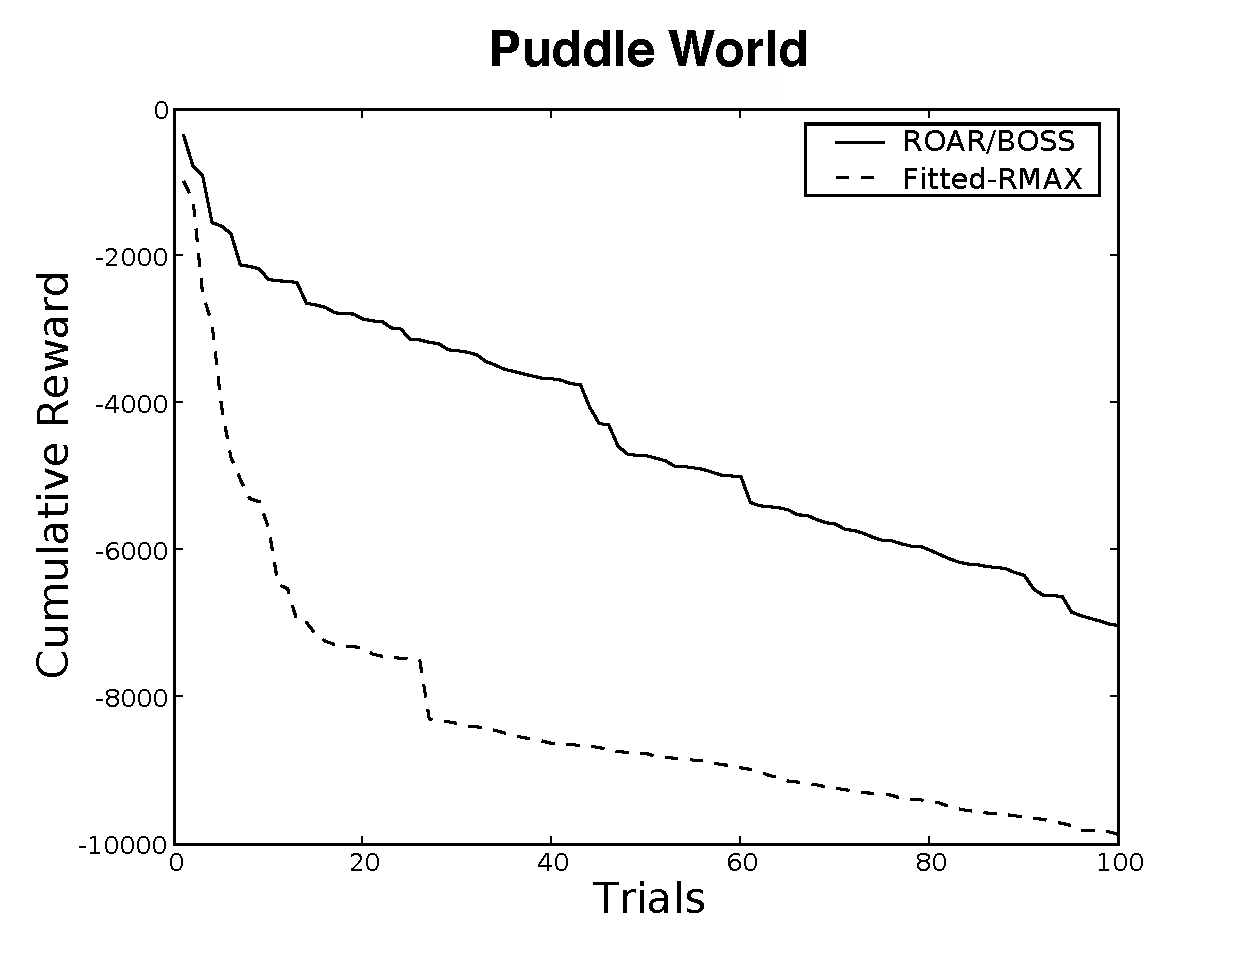
\includegraphics[width=\columnwidth]{puddleFigure}}
\caption{Typical of \alg{RMAX}-family algorithms, \alg{Fitted-RMAX} is very conservative, getting data from every portion of the environment before acting greedily. \prior{ROAR}/\alg{BOSS}, since it depends on posterior variance for exploration, starts getting good reward sooner, even though occasionally it decides to learn about a new area for a short period. \alg{Fitted-RMAX} was run with width parameter $b=0.05$ and knownness threshold $B=2$. \prior{ROAR}/\alg{BOSS} was run with $K=1, B=5, \alpha=1.0,\Psi_{\mbox s}=0.1I, m_{\mbox s}=200, \Psi_{\mbox o}=0.01I, m_{\mbox o}=30, \Psi_{\mbox r}=1.0I,m_{\mbox r}=20,\alpha_\phi=0.001,\beta_\phi=0.01$. Averaged over $20$ runs.}
\label{fig:puddle}
\end{center}
\vskip -0.2in
\end{figure} 


\subsection{\env{Bridge of Fire}}
\label{fire}

The previous sectionÊdescribed a model that is characterized as ``deterministic with small noise''. In the \env{Bridge of Fire} domain, this assumption is violated by making the noise associated with each action determine the action's effectiveness.

In the \env{Bridge of Fire} domain, the agent must navigate across a bridge, without falling off the side (and into the fire), using three actions corresponding to \emph{walk}, \emph{hand-spring} and \emph{pogo-stick}. \emph{Walk} is a very consistent action, moving the agent forward along the bridge with no lateral noise. \emph{Hand-spring} will move the agent faster, but there is a chance that the agent moves to one side or the other. \emph{Pogo-stick} will take the agent a long way, but there is a huge amount of uncertainty in the movement and more often than not the agent will pogo right off of the bridge.

More concretely, the bridge is a $2\times 10$ rectangle, and the agent begins in the middle of one edge. The \emph{walk} action moves the agent forward according to $N(0.5, 1)$ and sideways according to $N(0, 0)$. The \emph{hand-spring} action moves forward with $N(1,1)$ and sideways with $N(0,0.5)$, and finally the \emph{pogo-stick} action moves forward with $N(1.5,1)$ and sideways with $N(0,1)$. If the agent makes it to the other side of the bridge, it receives a reward of $100$ and the trial ends. If the agent falls, it receives a reward of $-100$ and the trial ends. Every non-terminal step gives the agent a reward of $-1$.

%[zzz ken says use covariance matrices instead of N(x,y)]

Ignoring the noise in the \env{Bridge of Fire} will cause the agent to prefer \emph{pogo-stick}, since the outcome moves the agent the furthest along the length of the bridge and has zero mean lateral displacement. In reality, the agent should prefer \emph{walk} until near the end, when \emph{hand-spring} becomes safer.

\prior{ROAR}/\alg{BOSS} is compared against \alg{Fitted-RMAX} and \alg{CORL} in Figure \ref{fig:bridge}.

\begin{figure}[t]
\vskip 0.2in
\begin{center}
\centerline{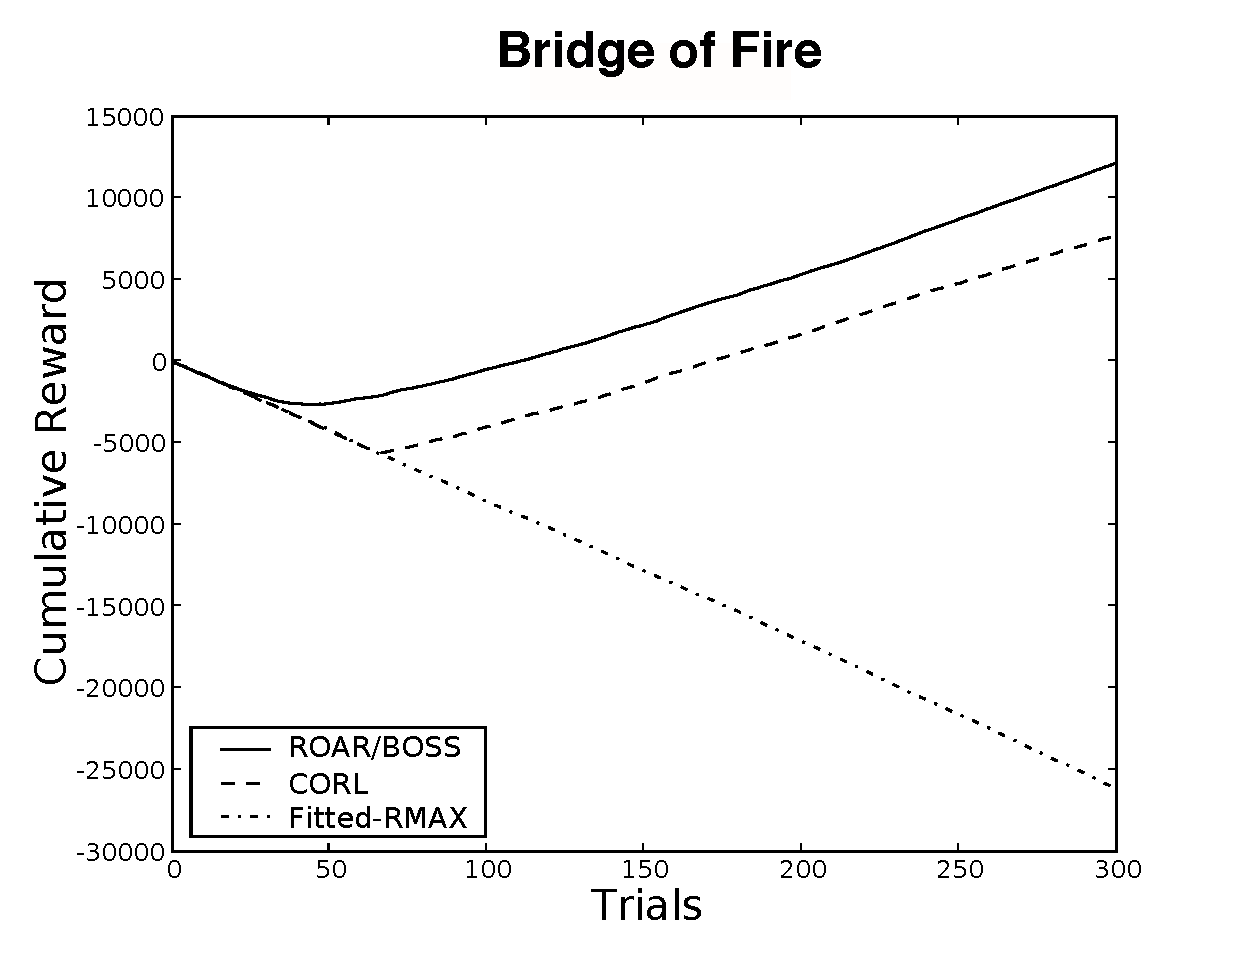
\includegraphics[width=\columnwidth]{bridgeFigure}}
\caption{Algorithms using \prior{ROAR} and \alg{CORL} were able to learn the \env{Bridge of Fire} domain effectively. \alg{Fitted-RMAX} makes assumptions that do not hold in this environment, and does poorly as a result. \alg{CORL} was run with knownness threshold $B=20$, and was given the correct type function. \alg{Fitted-RMAX} was run with width parameter $b=0.5$ and knownness threshold $B=3$. \prior{ROAR}/\alg{BOSS} was run with $K=1, B=10, \alpha=1.0,\Psi_{\mbox s}=0.1I, m_{\mbox s}=3, \Psi_{\mbox o}=0.1I, m_{\mbox o}=3, \Psi_{\mbox r}=1.0I,m_{\mbox r}=50,\alpha_\phi=0.001,\beta_\phi=0.005$. Averaged over $20$ runs.}
\label{fig:bridge}
\end{center}
\vskip -0.2in
\end{figure} 

\subsection{Mind the Gap}
\label{gap}

The \env{Mind the Gap} domain is similar to \env{Bridge of Fire}, except none of the actions have lateral displacement; the agent always goes straight and will never fall off the side. However, beginning $5$ units from the beginning, there is a $1$ unit stretch where the bridge has given out. To compensate, the agent has become better at the using the \emph{pogo-stick} action: The agent will either remain still or move forward exactly $1.5$ units. The \emph{pogo-stick} action becomes appropriate when the agent is within $0.5$ units of the gap, though due to noise in the other actions, it is still very difficult to avoid the gap with high probability.

The correct model in \env{Mind the Gap} is very difficult to learn. Using \prior{ROAR} with \alg{Bayesian~DP} proved ineffective; sampling only a single model at a time didn't give the agent enough reason to learn sufficiently about some parts of the state space. However, using \alg{BOSS} as the sampler was more successful. \alg{BOSS} is a very conservative algorithm, ``pooling'' the optimism from each of its sampled models for planning. This domain demonstrates the need for such optimism.

\prior{ROAR}/\alg{BOSS} and \prior{ROAR}/\alg{Bayesian~DP} are compared against \alg{CORL} in Figure \ref{fig:bridge2}.

\begin{figure}[t]
\vskip 0.2in
\begin{center}
\centerline{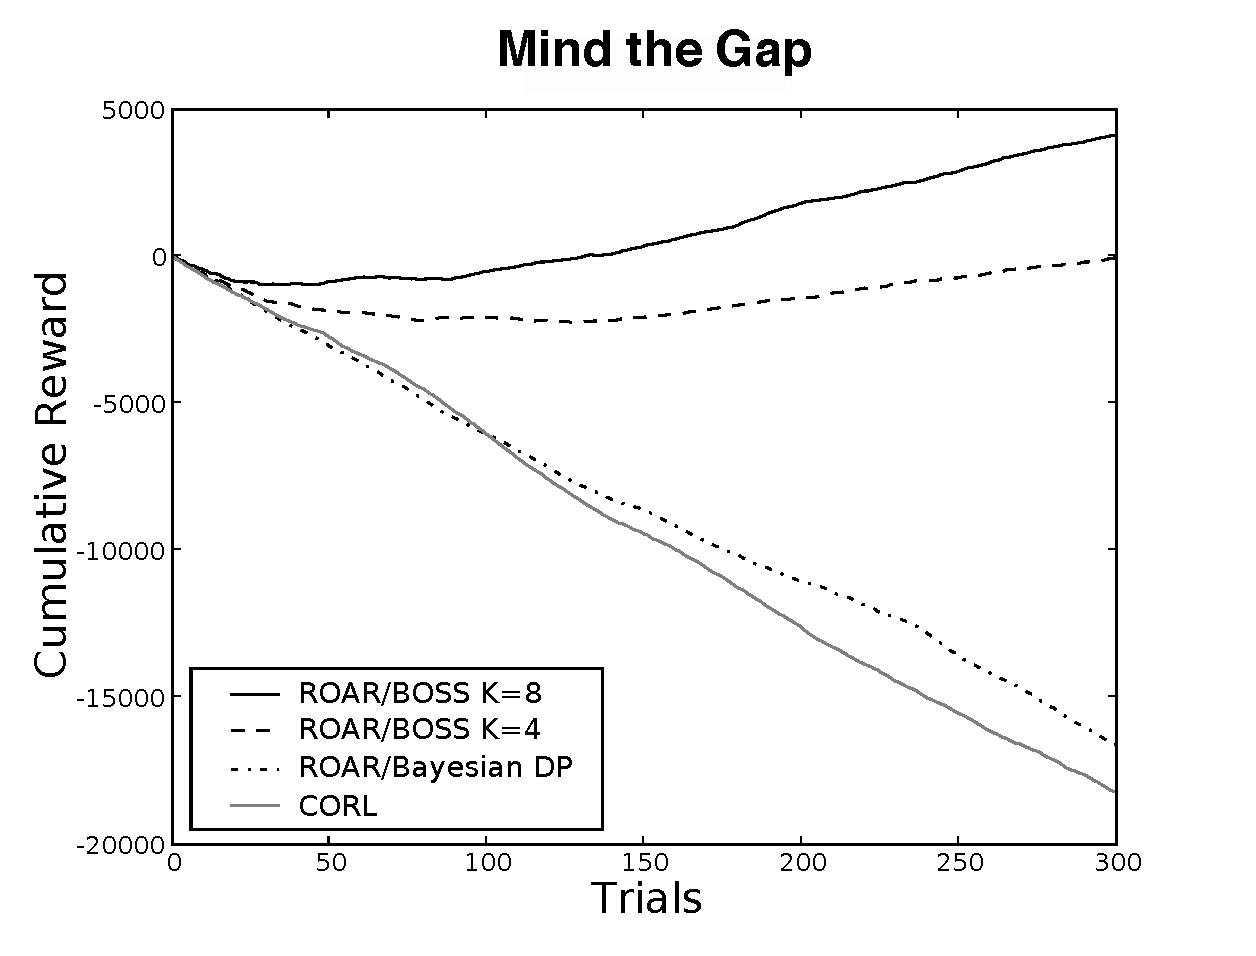
\includegraphics[width=\columnwidth]{bridge2Figure}}
\caption{Because of its unimodal outcome distribution assumption, \alg{CORL} was unable to perform well in the \env{Mind the Gap} domain, even after being told the correct ``type'' function for clustering. \prior{ROAR}, with no prior knowledge of the clustering, is able to effectively learn multi-modal distributions and can correctly model this environment's dynamics. \alg{CORL} was run with knownness threshold $B=10$. \prior{ROAR} algorithms were run with $B=1, \alpha=1.0,\Psi_{\mbox s}=0.5I, m_{\mbox s}=10, \Psi_{\mbox o}=0.1I, m_{\mbox o}=3, \Psi_{\mbox r}=0.01I,m_{\mbox r}=50,\alpha_\phi=0.01,\beta_\phi=0.001$. \prior{ROAR}/\alg{Bayesian~DP} drew samples every $20$ steps. Averaged over $20$ runs.}
\label{fig:bridge2}
\end{center}
\vskip -0.2in
\end{figure} 






\section{BFS3 experiments}

To demonstrate \alg{BFS3}, we will show its performance in a number of domains, and show how the use of different priors can affect its performance.  This flexibility with respect to using different priors is a compelling reason to use MCTS algorithms in general, and \alg{BFS3} in particular, for model-based reinforcement learning.

The first experiment is very simple, and exact Bayes-optimal behavior is possible. \env{Bernoulli-bandits} is a $5$-armed bandit problem where each arm $a$ has some unknown probability $p_a \sim Beta(\alpha,\beta)$ of returning a reward of $1$ or $0$ each step. For each run in the experiment, the environment parameters $p_a$ are drawn directly from the prior. The Gittins Index~\cite{gittins89} can be used to achieve Bayes-optimal behavior for multi-armed bandit problems. After $1000$ steps, \alg{BFS3} with the true prior received an average (over 40 runs) total reward of $727$, where the Bayes-optimal agent received an average total reward of $815$.

% zzz ML: Can you say how many steps were not approximately Bayes optimal?
% zzz ML: What were t and C?  (or any other relevant parameters)
% zzz ML: What does BEB do?

When using the \prior{FDM} prior with a small state space, \alg{BEB} may be considered a better choice. Since \alg{BEB} operates greedily according to a grounded MDP, rather than a belief-MDP,  planning is made potentially much easier. This algorithm is limited, however, in that it requires a known reward function; it can only deal with uncertainty in the transition function.

\alg{BFS3}, with the right prior, can handle unknown rewards. In many domains, there are only a few possible reward values. For example, many path-finding domains give a reward of $-1$ for all actions. Or, there is a reward for a particular outcome that can be achieved from multiple states: these states would share the same reward value.  To represent this common structure in a generative model, the Dirichlet Process (DP)~\cite{maceachern98} may be used:
\begin{eqnarray*}
R_{s,a} &\sim& \mbox{DP}(\alpha, \mbox{Unif}(\Rmin, \Rmax)).
\end{eqnarray*}
Note that with this prior, rewards are deterministic, if unknown.
% zzz ML: what parameter used in Rmax?

In Figure~\ref{fig:grids}, \alg{BFS3}, with the unknown reward prior, is shown to suffer no significant performance penalty compared to \alg{BFS3} with the known-reward prior and to \alg{BEB} (which also uses the known-reward prior). The domain is a $5\times 5$ grid world, where the agent must find its way from one corner to the other. The agent can choose to go north, east, south or west, and with probability $0.2$ it will go in a direction perpendicular to the one intended.
% zzz ML: what of computation time?  how much worse is BFS3?



\begin{figure}
\vskip 0.2in
\begin{center}
\centerline{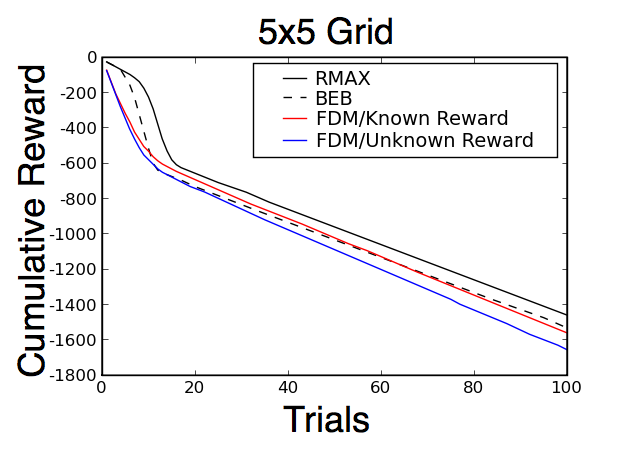
\includegraphics[width=3in]{grids}}
\caption{
Here \alg{BFS3}/\prior{FDM}, with both known rewards and unknown rewards with a DP prior, is compared against the known-reward \alg{BEB}, and \alg{RMAX}~\cite{brafman02}, a well known algorithm with PAC-MDP guarantees, with $M=5$. Results are averaged over $40$ runs.
}
\label{fig:grids}
\end{center}
\vskip -0.2in
\end{figure} 

Along with \prior{FDM}, we introduce the \prior{Factored-Object} prior, which describes factored MDPs in which the state features are broken up into a number of independent yet identical objects. The action also has two features: the first indicates which object is being acted upon, and the second indicates which action is being performed. \prior{Factored-Object} essentially has a single \prior{FDM} posterior, which it applies to each object in the state simultaneously, sharing both information (for faster convergence) and memory.

%In Figure~\ref{fig:dgms}, we show the plate diagram representing these two priors. 

For a single object, \prior{Factored-Object} and \prior{FDM} are the same. For two objects, \prior{FDM} has to learn separately how a particular action affects a particular object for every possible configuration of objects---for a different state of an object not being operated on, \prior{FDM} must re-learn how the original object is affected. \prior{Factored-Object} allows the agent to learn about multiple objects at the same time: it knows that a given action affects object $1$ in the same way it affects object $2$, and generalizes appropriately.

The Paint/Polish world~\cite{walsh09a} provides a situation where the simple and convenient \prior{FDM} prior is insufficient. The size of the state-space grows exponentially with the number of cans to paint (each of which introduces four binary features). Figure~\ref{fig:paint1-2can} shows the results with a single can (and $2^4$ states) and the results with two cans (and $2^{4\cdot 2}$ states). Figure~\ref{fig:paint4can} shows the results with four cans (and ${2^4}^4$ states).


%%
\begin{figure}
\vskip 0.2in
\begin{center}
\centerline{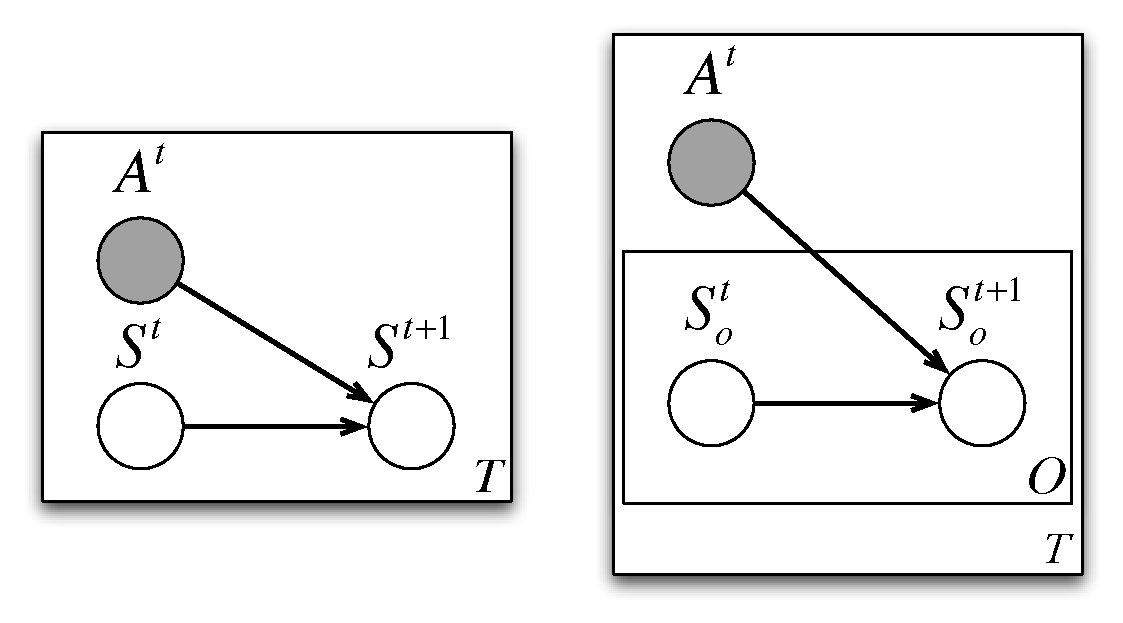
\includegraphics[width=3in]{dgms}}
\caption{
The Directed Graphical Models for \prior{FDM} (left) and \prior{Factored-Object} (right). Nodes indicate random variables, and edges show possible dependencies. Shaded nodes are observed. Boxes indicate repetition.
}
\label{fig:dgms}
\end{center}
\vskip -0.2in
\end{figure} 

\begin{figure}
\vskip 0.2in
\begin{center}
\centerline{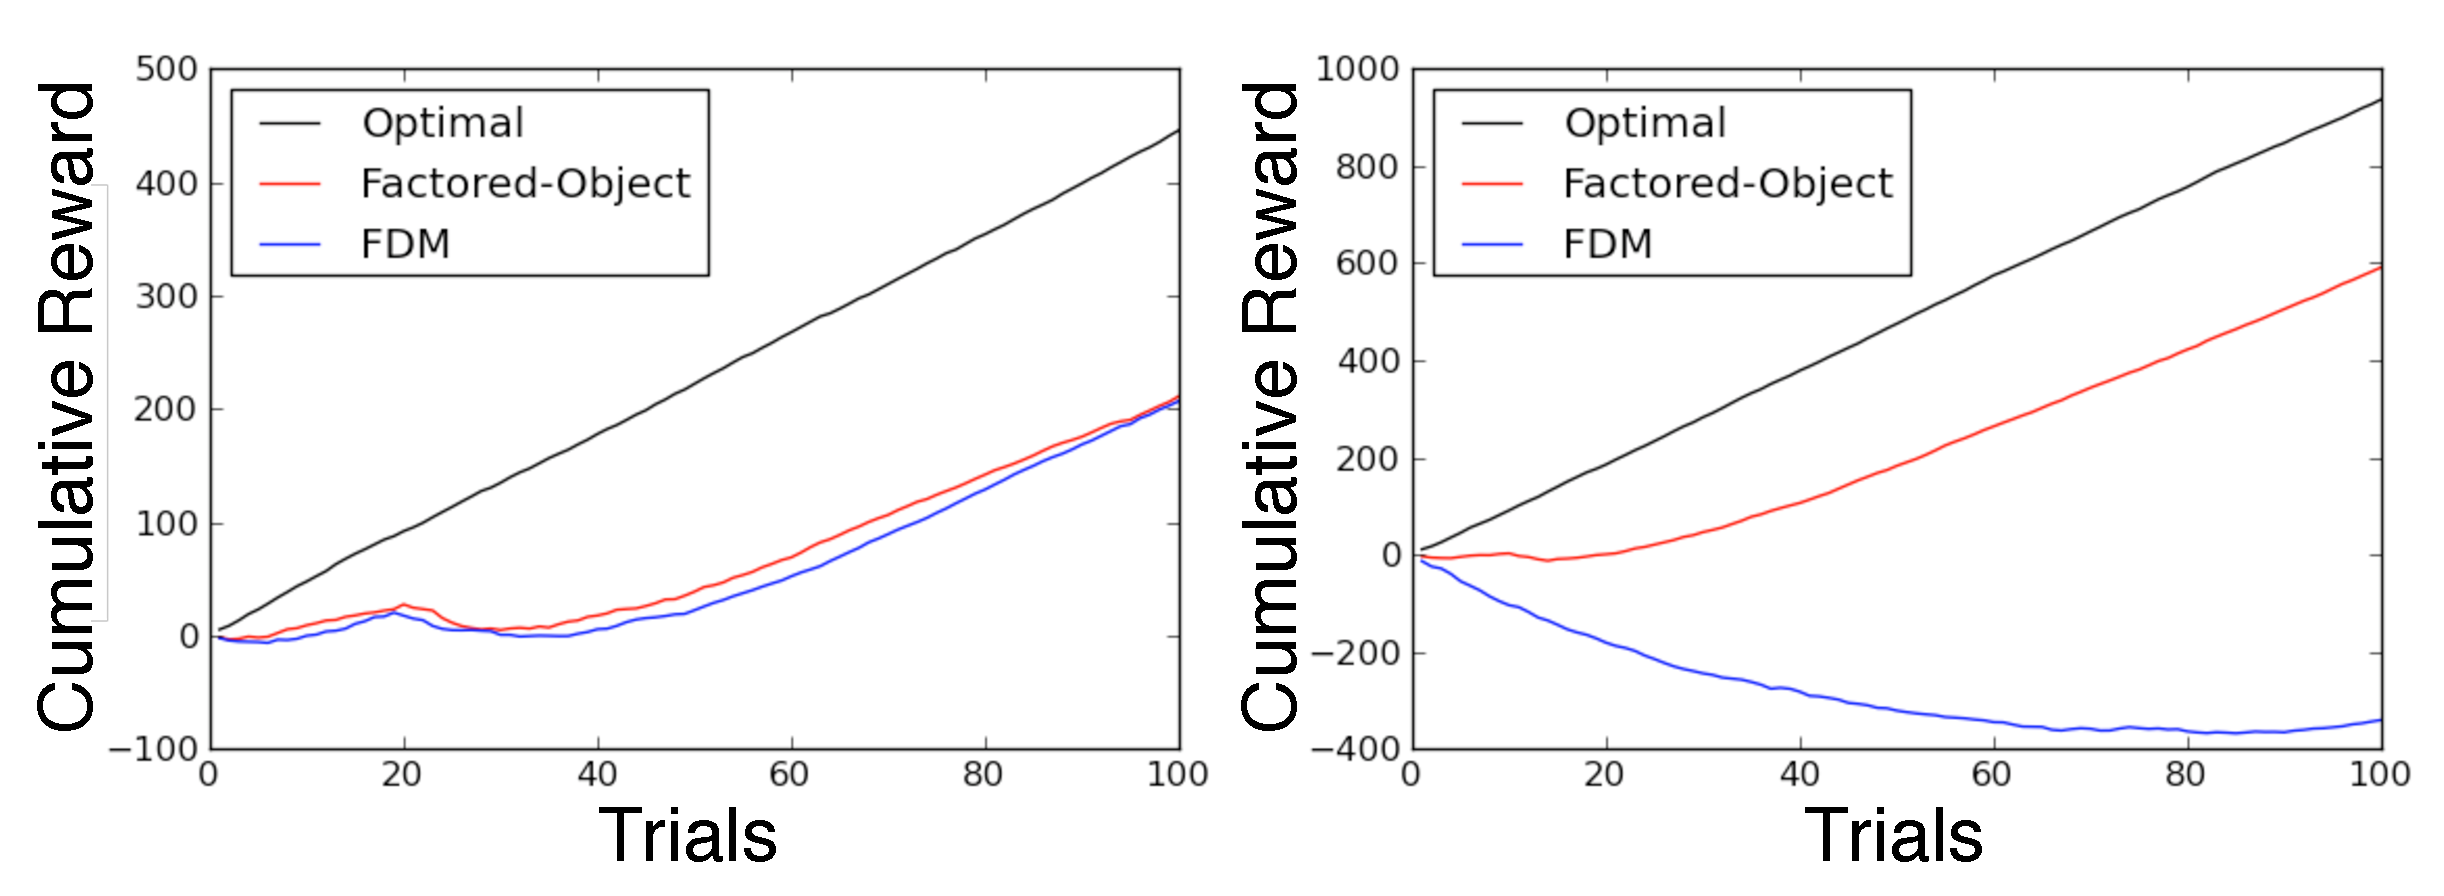
\includegraphics[width=3in]{paint1-2can}}
\caption{
\alg{BFS3} with \prior{FDM} and \prior{Factored-Object} priors. {\bf Left:}~Paint/Polish with 1 can. \prior{FDM} and \prior{Factored-Object} are identical for one object, and give the same performance. {\bf Right:}~Paint/Polish with 2 cans. \prior{Factored-Object} outperforms \prior{FDM} because it is better able to generalize. Results are averaged over $40$ runs.
}
\label{fig:paint1-2can}
\end{center}
\vskip -0.2in
\end{figure} 

% zzz ML: error bars?

\begin{figure}
\vskip 0.2in
\begin{center}
\centerline{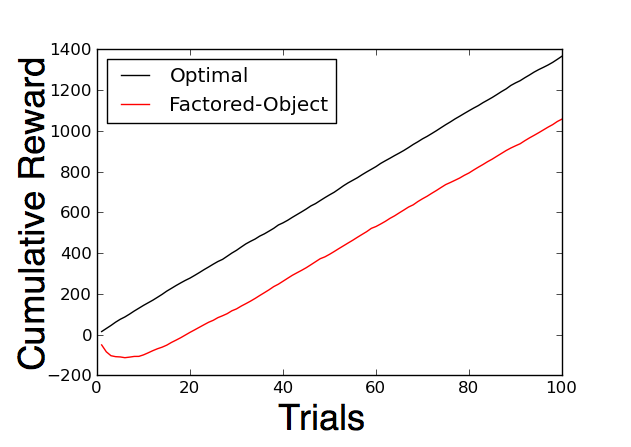
\includegraphics[width=3in]{paint4can}}
\caption{
Paint/Polish with 4 cans. Using the \prior{Factored-Object} prior allows \alg{BFS3} to learn quickly despite the very large state space. Using \prior{FDM} does not allow learning in a reasonable amount of time, and is not pictured. Results are averaged over $40$ runs.
}
\label{fig:paint4can}
\end{center}
\vskip -0.2in
\end{figure} 


\subsection{Wumpus World}

\alg{BFS3} can also be used to apply Bayesian modeling to POMDPs. \env{Wumpus World}~\cite{russell94} is based on a classic computer game in which an agent wanders through a $4\times 4$ maze filled with fog, making it impossible to see past its current cell. Even though the agent cannot see, it can feel a breeze if there is a pit in an adjacent cell, and smell a stench if there is a Wumpus\footnote{A Wumpus is a monster that eats RL agents.} near-by. If the agent falls into a pit, it will remain there forever. If the agent runs into the Wumpus, it is eaten. If the agent shoots its one arrow in the direction of the Wumpus, the Wumpus is slain. If the arrow misses the Wumpus, the trial ends and presumably the agent goes home. We replicate the dynamics presented in detail by Sorg et al. (2010). % zzz noun cite

\env{Wumpus World} is based on a deterministic process, but since the agent only knows attributes of cells that it has visited, it appears stochastic. The prior over different possible mazes is known and given to the agent, and from this it can infer the correct posterior distribution over what happens when it performs a particular action in a particular belief-state.

We ran \alg{BFS3} on \env{Wumpus World} with a search depth of $15$, and varied the number of trajectories per step. Agents with $500$, $1000$, and $5000$ trajectories per step averaged $0.267$, $0.358$ and $0.499$ cumulative reward, respectively. Averages were taken over $1000$ attempts. We compare this to a variance-based reward bonus strategy~\cite{sorg10} which, when tuned, averaged $0.508$.

That \alg{BFS3} performs better in \env{Wumpus World} as the computation budget is increased supports our argument that the algorithm has a \emph{computational resources} knob which, when tuned higher, causes the agent's behavior to get closer to being Bayes-optimal at the cost of decision-making speed.

%
\ifperchapterbib%
For the convenience of the reader, a list of references is provided at the end of each chapter (where applicable).
\ifendbib%
%A bibliography containing all cited references is included at the \hyperref[sec:bibliography]{end of the dissertation}.
\else\fi% end ifendbib
%\cbend%
\else\fi% end ifperchapterbib
